\section{网络的牵制控制研究}

本章从牵制控制的动力学模型出发,引出衡量网络控制能力的经典比率判据。因为传统比率判据无法精确衡量网络的牵制控制能力,本章提出耦合强度范围和收敛速度两个指标。
这两个指标由作者原创提出,前者决定了网络牵制控制时模型中耦合强度的大小,后者则从李雅普诺夫指数方面,给出了网络控制速度。
耦合强度范围和收敛速度完全不同,他们分别从不同角度刻画了网络牵制控制。
另外,实验还发现传统判据、耦合强度范围和收敛速度这三个指标无法同时到达最优状态。

\subsection{网络的牵制控制}
\subsubsection{稳定性分析}

在章节\ref{Sec: control} 中,动力学方程\ref{Eq:all_dynamical} 描述了牵制控制中控制节点和普通节点的动力学演化过程。
另外,网络也是一个混沌系统,混沌系统的特点是对初值极为敏感,两个极为接近的初始值随时间的变化,其产生的轨道会按照指数幂进行分离,通常用李雅普诺夫指数这个参数来描述这种现象 \cite{Wolf1985}。
为了使节点最终到达的状态得到稳定,现在从结果出发,考虑把网络控制在一个平衡点$\overline{\textbf{x}} = (\overline{x}_1, \overline{x}_2, ..., \overline{x}_n)^T$,则方程\ref{Eq:all_dynamical} 可转化为 \cite{汪小帆2006}:
\begin{equation}
\dot{\xi}_i = [Df+c{\lambda}_iH]{\xi}_i,\quad i=1,2,..,N
\label{Eq: Reduce_MSF}.
\end{equation}
其中,$ Df $代表节点自身演化函数$ f $的雅可比矩阵,$ \xi_i $代表节点状态$x_i$转化后的状态变量,$ {\lambda}_i $代表牵制控制矩阵$ C $ 的特征值,且有$ 0 > {\lambda}_1 \geq {\lambda}_2 \geq ... \geq {\lambda}_N$。$ C=-L-D $,$ D $ 为对角阵 $ D=diag\{d_1,d_2,...,d_N\} $。其中,如果节点$ i $是一个控制节点,则 $ d_i=d $,否则,$ d_i=0 $。牵制控制矩阵$ C $可描述为:
\begin{equation}
C=
\left[
\begin{matrix}
-l_{11}-d_1      & -l_{12}       & \cdots & -l_{1N}       \\
-l_{21}       & -l_{22} -d_2      & \cdots & -l_{2N}      \\
\vdots & \vdots & \ddots & \vdots \\
-l_{N1}       & -l_{N2}       & \cdots & -l_{NN}-d_N       \\
\end{matrix}
\right].
\label{Eq: C}
\end{equation}

考虑式子\ref{Eq: Reduce_MSF}的广义函数,可以得到主稳定方程 \cite{Sorrentino2007}:
\begin{equation}
\dot{y} = [Df + \alpha H]y.
\label{Eq: MSF}
\end{equation}
该方程的最大李雅普诺夫指数$ L_{max} $是关于实数变量$ \alpha $的函数。假设实数变量$ \alpha \in (\alpha_2, \alpha_1) $,由式子\ref{Eq: Reduce_MSF} ,有$ \alpha_2 <c\lambda_i<\alpha_1 $。

在控制理论中,雅普诺夫指数也是衡量系统能否稳定的重要指标。一个混沌系统的最大李雅普诺夫指数大于$ 0 $,代表这个系统中,无论两个轨道的初始间距多么微小,这两个轨道终会随时间而呈指数发散而无法观测。
反之,若一个系统的最大李雅普诺夫指数小于$ 0 $,则这个系统某初始状态可能会收敛,即两个不同的轨道可能会随时间而发生重叠。
因此要使得整个系统稳定,最大李雅普诺夫指数$ L_{max} $必须小于0,即:
\begin{equation}
\Lambda_{max}[Df + \alpha H]<0.
\label{Eq:princple_eigenvalue}
\end{equation}
其中,$ \Lambda_{max} $ 为$ [Df + \alpha H] $的最大特征值。

本节分析了平衡点的局部稳定状态,通过最大李雅普诺夫指数是否小于$ 0 $,来判断平衡点是否能稳定。平衡点能稳定,代表网络有机会得到控制。
因此,最大李雅普诺夫指数小于$ 0 $是网络受控的必要非充分条件。网络得到控制,则该系统的最大李雅普诺夫指数小于$ 0 $;但是,最大李雅普诺夫指数小于$ 0 $不一定意味着网络能够得到控制。
就目前而言,采用李雅普诺夫指数是计算复杂网络牵制控制的最佳方法。


\subsubsection{经典比率判据}
根据主稳定方程\ref{Eq: MSF},最大李雅普诺夫指数是关于实数变量$ \alpha $的函数。
因此通过$ \alpha $的取值范围,网络的牵制控制可以分为三个方面来考虑 \cite{汪小帆2006}:

(1) $ \alpha \in S1 = (-\infty,\alpha_2) $,且 $ \alpha_2 $是一个负实数。
在这种情况下,为了确保控制的稳定状态,只需要有:
\begin{equation}
c\lambda_1<\alpha_2.
\end{equation}
此时,节点对网络的控制强度由$ \lambda_1 $来决定。$ \lambda_1 $越小,耦合强度$ c $的取值范围也就越大,网络也就更容易达到受到控制。

(2) $ \alpha \in S2 = (\alpha_2, \alpha_1) $,且 $ \alpha_2<\alpha_1<0 $。
在这种情况下,为了控制确保稳定状态,耦合强度需要满足不等式:
\begin{equation}
\alpha_2<c\lambda_N,
c\lambda_1<\alpha_1.
\label{Eq: coupling_strength}
\end{equation}
在耦合强度满足以上关系时,该网络的受控状态是渐进稳定的。
通常而言,公式\ref{Eq: coupling_strength}被当作网络牵制控制比例判据,并定义:
\begin{equation}
R = \frac{\lambda_1}{\lambda_N} > \frac{\alpha_1}{\alpha_2}.
\label{Eq: R}
\end{equation}
$ R $称之为经典比率判据,其只与网络自身的拓扑结构和控制节点有关。
$ R $值越大,代表节点对网络的控制能力也就越强。

(3) $ S3 = \emptyset $。在这种情况下,网络无法得到控制。在本文中,不考虑这种情况。

\subsection{耦合强度范围与收敛速度}
事实上,经典比率判据$ R $无法精确衡量节点对网络的牵制控制能力,在极端情况下,$ R $会失效。因此,本节针对于网络牵制控制问题,将节点对网络的牵制控制能力可以分为两个部分:耦合强度范围和网络的收敛速度。
耦合强度范围由比例判据而来,指明了要使网络得到控制,耦合强度需要满足的条件;
收敛速度即网络受控稳定的速度,其与主稳定方程的最大李雅普诺夫指数有关。
耦合强度范围和收敛速度由作者原创,这两者分别从不同角度刻画了网络牵制控制的情况,关联性极低。

\subsubsection{耦合强度范围}
为了控制一个网络,使之到达稳定的状态,耦合强度必须满足公式 \ref{Eq: coupling_strength} 。因此,耦合强度范围定义为:
\begin{equation}
\omega = \frac{\alpha_2}{\lambda_N} - \frac{\alpha_1}{\lambda_1} >0.
\label{Eq: omega}
\end{equation}
很明显,耦合强度范围为耦合强度满足控制条件的差值。
节点之间耦合强度可供选择的范围越大,也就更容易找到一个合适的耦合强度的值来促使网络到达受控稳定状态。
因此,同经典判据一样,耦合强度范围也越大越好。
为了使耦合强度范围更大,研究人员可以采用不同的重要节点检测算法,来获取网络的牵制控制节点。

需要注意到的是,经典判据$ R $和耦合强度$ \omega $是两个完全不同的衡量标准。
经典判据$ R $只依赖于网络的拓扑结构,不同牵制控制节点的选择会影响特征值$ \lambda_1 $和$ \lambda_N $,从而影响判据$ R $的变化。
但耦合强度范围$ \omega $还与常数$ \alpha_1 $和$ \alpha_2 $的值有关。
一般而言,不同的网络模型、节点自身不同的演化函数$ f(x) $、节点间的不同的耦合方式$ H $都影响着$ \alpha_1 $和$ \alpha_2 $的取值。
在$ \alpha_1 $和$ \alpha_2 $确定后,牵制节点再通过影响特征值$ \lambda_1 $和$ \lambda_N $,来影响耦合强度范围$ \omega $。
直观而言,在控制节点确定时,更大的比例判据$ R $通常意味着更小的$ \alpha_1 $和更大的$ \alpha_2 $,而这两者会导致耦合强度范围$ \omega $的增加。但是,比例判据$ R $和耦合强度范围$ \omega $不存在严格意义上的等价关系,两者是完全不同的衡量网络控制能力的评判标准。

\subsubsection{收敛速度}
当牵制节点控制一个网络时,另一个需要考虑的问题是系统达到稳定状态时的速度,称之为收敛速度。
严格来说,网络的收敛速度由方程 \ref{Eq: Reduce_MSF} 中$( Df+c{\lambda}_iH) $的最大特征值所决定,即$ \Lambda_{max}[Df + c{\lambda}_i H] $。
在标准控制理论中,$ \Lambda_{max}[Df + c{\lambda}_i H] $指的也是最大李雅普诺夫指数。
%同时,在主稳定方程 \ref{Eq: MSF} 中提到,最大李雅普诺夫指数是关于$ \alpha $的函数,
在大部分真实系统中,关于$ \alpha $的函数$ \Lambda_{max}[Df + \alpha H] $只有一个最小值,比如说罗塞尔吸引子、洛
伦兹吸引子 \cite{Stewart2000} 和陈氏吸引子 \cite{L2002} 等。
因此,网络的收敛速度可以简化成比较矩阵$ (Df+c\lambda_1H) $和矩阵$ (Df+c\lambda_NH) $的最大特征值。于是,收敛速度定义为:
\begin{equation}
v = max\{\Lambda_{max}[Df+c\lambda_1H],\Lambda_{max}[Df+c\lambda_NH]\}.
\end{equation}

同时,$ v $也代表整个系统动力学方程\ref{Eq:all_dynamical} 的最大李雅普诺夫指数$ L_{max} $。
控制理论中,$ L_{max}<0 $是系统到达稳定状态的必要不充分条件。
因此,要使节点对网络的控制达到稳定状态,必须保证$ L_{max}<0 $,即$ v<0 $;
反之在$ v>0 $的情况下,该系统是无法到达稳定状态的。
在牵制控制节点数目确定时,如果要使网络更快地到达稳定状态,就需要最小化收敛速度$ v $。
也就是说,更小的收敛速度$ v $意味着更小的最大李雅普诺夫指数$ L_{max} $,网络也就能更快地得到稳定控制。

\subsubsection{三个指标的微分分析}
假设某个网络$ G = (V, E) $已经被部分牵制控制节点所控制,反馈强度为$ d $。当网络中新增一个节点$ i $到牵制控制节点集合中时,节点$ i $所引起的牵制控制矩阵$ C $的变化为:$C'=C-\Delta D$。其中,$\Delta D=diag\{0,...,0,d_i,0,...,0\}$,$ \Delta D $只有一个非$ 0 $元素$ d_i $。矩阵$ C' $的特征值$ \lambda_k' $和对之对应的特征向量$ X_k' $变化为:$\lambda_k'=\lambda_k+\Delta{\lambda_k}$,$X_k'=X_k+\Delta{X_k}$,且满足:
\begin{equation}
(-L-D-\Delta{D})(X_k+\Delta{X_k}) = (\lambda_k+\Delta{\lambda_k})(X_k+\Delta{X_k}).
\label{Eq: single_driver}
\end{equation}
两边同时左乘$ X_k^T $,忽略二阶导数项$ \Delta{D}\Delta{X_k} $和$ \Delta{\lambda_k}\Delta{X_k} $,可以得到:
\begin{equation}
\frac{\partial\lambda_k}{\partial{d_i}} = -(X_k^i)^2,
\label{Eq: Lambda_eigenvector}
\end{equation}
其中,$ X_k^i $代表的是特征向量$ X_k $的第$ i $个元素。
式子\ref{Eq: Lambda_eigenvector}将特征值$ \lambda_k $对节点的反馈$ d_i $,简化成特征值$ \lambda_k $所对应特征向量$ X_k $的变化情况。

对于传统判据$ R $而言,当新增一个节点$ i $作为控制节点时,传统判据对节点$ i $的微分为:
\begin{equation}
\begin{aligned}
\frac{\partial R}{\partial di} &= \frac{\partial}{\partial di}(\frac{\lambda_1}{\lambda_N})
\\
&= \frac{\lambda_N\frac{\partial \lambda_1}{\partial di}-\lambda_1\frac{\partial \lambda_N}{\partial di}}{\lambda_N^2}
\end{aligned}
\label{Eq: ddR}
\end{equation}

将式子 \ref{Eq: Lambda_eigenvector} 代入式子 \ref{Eq: ddR} ,可以得到:

\begin{equation}
\begin{aligned}
\frac{\partial R}{\partial di} &= -\frac{ \lambda_N(X_1^i)^2 - \lambda_1(X_N^i)^2}{\lambda_N^2}
\\
&=-\frac{1}{\lambda_N}[(X_1^i)^2-R(X_N^i)^2].
\end{aligned}
\label{Eq: dR}
\end{equation}
其中,$ X_1 $与$ X_N $分别是牵制控制矩阵$ C $的最大、最小特征值$ \lambda_1 $和$ \lambda_N $所对应的特征向量,$ R $为添加控制节点$ i $前原始控制节点对网络控制的经典比率判据。

同理,对耦合强度范围而言,当新增节点$ i $作为牵制控制节点时,耦合强度范围对该节点的微分为:
\begin{equation}
\begin{aligned}
\frac{\partial \omega}{\partial{d_{i}}} &= \frac{\partial}{\partial di}(\frac{\alpha_1}{\lambda_1}) - \frac{\partial}{\partial di}(\frac{\alpha_2}{\lambda_N})
\\
&=\frac{1}{\lambda_1^2}(\alpha_1\frac{\partial \lambda_1}{\partial d_i} - \alpha_2\frac{\lambda_1^2}{\lambda_N^2}\frac{\partial\lambda_N}{\partial d_i})
\\
&= -\frac{1}{\lambda_1^2}[\alpha_1(X_1^i)^2-\alpha_2R^2(X_N^i)^2].
\end{aligned}
\label{Eq:orginperturb2}
\end{equation}

相应地,收敛速度$ v $对新增牵制控制节点$ i $的微分为:
\begin{equation}
\frac{\partial v}{\partial di}=max\{-c\frac{dF(\rho)}{d\rho}(X_1^i)^2,-c\frac{dF(\rho)}{d\rho}(X_N^i)^2\}.
\label{Eq: dv}
\end{equation}
其中,$ dF(\rho) = \Lambda_{max}[Df+\rho H] $。当$ F(c\lambda_1)>F(c\lambda_N)$时,该微分取$ -c\frac{dF(\rho)}{d\rho}(X_1^i)^2 $;当$ F(c\lambda_1)<F(c\lambda_N)$时,该微分为$ -c\frac{dF(\rho)}{d\rho}(X_N^i)^2 $。

通过传统比率判据的微分(\ref{Eq: dR}),耦合强度范围的微分(式子\ref{Eq:orginperturb2})以及网络收敛速度的微分(\ref{Eq: dv}),不难发现在网络中新增一个控制节点时,传统判据、耦合强度范围和收敛速度增加的值也有所不同,这说明了这三个指标分别从不同的角度描述了网络的牵制控制问题。同时,三个指标中某一个指标的增加,可能会导致另外指标的减少。因此,这三个指标无法同时到达最优状态。

\subsection{实验模拟}
为了将传统判据、耦合强度范围和收敛速度这三个指标区分开,实验先在经典的空手道俱乐部网络上做了示例说明;然后,在4个真实网络中,在不同的控制节点比例下,分别最优化传统判据、耦合强度范围和收敛速度,穷举获得不同的控制节点集合,观察在不同控制集合下这三个指标的变化过程。

\subsubsection{空手道网络的示例}

\begin{figure}[ht]%{.5\linewidth}
	\centering
	% Requires \usepackage{graphicx}
	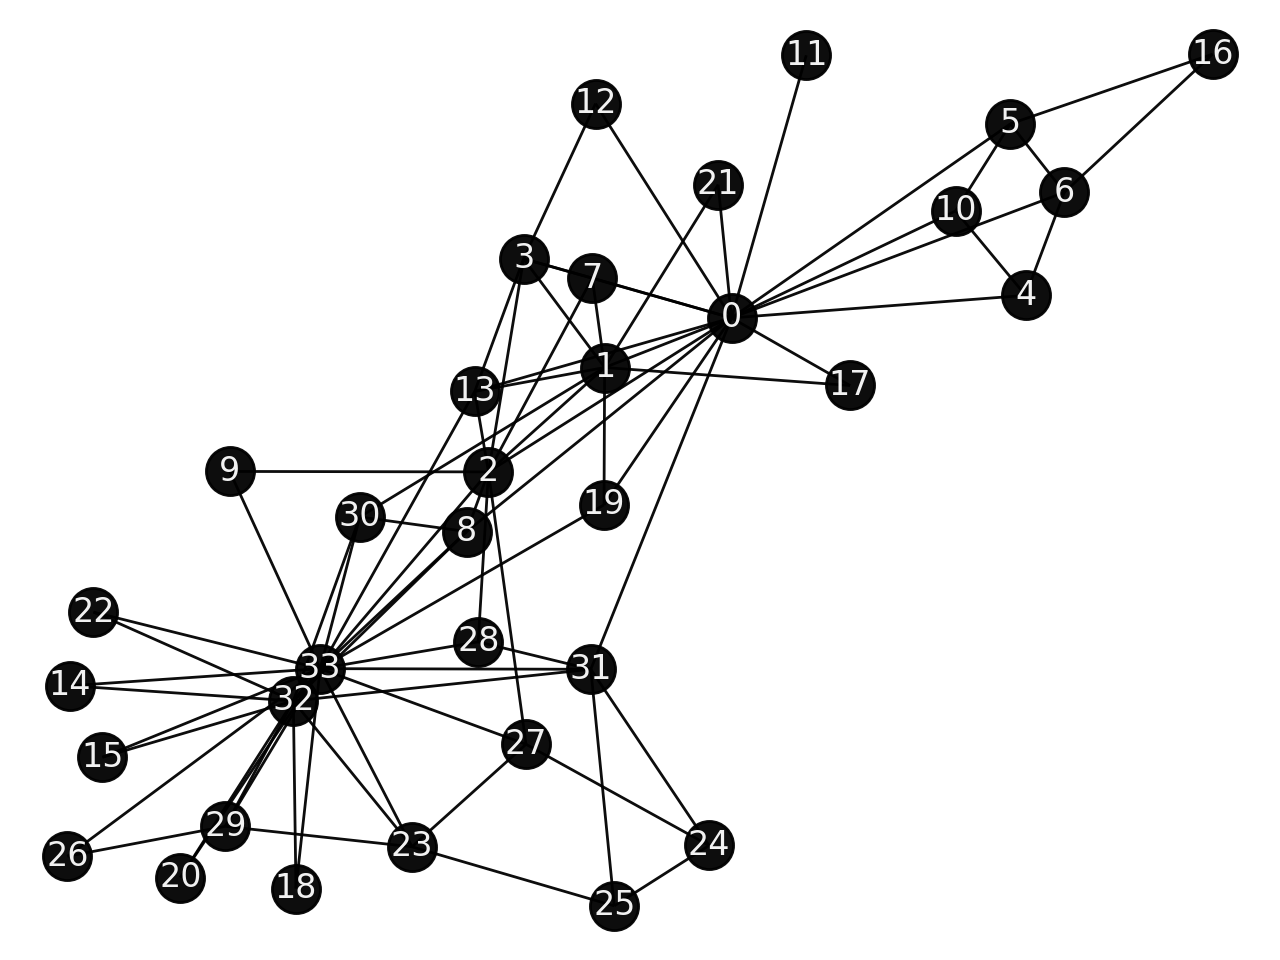
\includegraphics[width=0.6\columnwidth]{chapter3Fig/exm.png}\\
	% 
	\caption{空手道俱乐部网络}
	\label{Fig: karate}	
\end{figure}

图 \ref{Fig: karate} 是经典的空手道俱乐部网络Zachary  \cite{Zachary1977} 。该网络由34个节点构成,节点间有78条连边。
网络中,节点代表空手道俱乐部成员,节点之间的连边代表俱乐部成员之间存在某种关系。在这个网络上,实验分别最优化经典判据$ R $,耦合强度范围$ \omega $和收敛速度$ v $,穷举破解得到5个牵制控制节点;并观察分别在不同控制节点集合下,这三个指标的变化情况。实验参数设置见章节$ 3.3.3 $。

\begin{table*}[h]\centering{	
		\caption{不同的牵制节点对应三种指标的变化情况}
		\centering
		{	\begin{tabular}{cccc}
				\hline
				\hline
				 &Optimal $ R $&Optimal $ \omega $&Optimal $ v $\\ \hline
		  控制节点&[1,2,5,31,32]&[0,2,6,32,33]&[4,13,16,25,26] \\
			$ R $&\textbf{0.026} &0.025&0.015 \\
	   $ \omega $&-0.106&\textbf{-0.080}&-0.352\\
			$ v $&0.086&0.102&\textbf{0.047} \\
				\hline
				\hline	
			\end{tabular}				
			\label{table:exm}
	}}
\end{table*}

表 \ref{table:exm} 描述了不同的牵制节点对应的三种指标的变化情况。实验通过最优化传统判据$ R $,耦合强度范围$ \omega $和收敛速度$ v $,分别得到的不同的控制节点集合$ [1,2,5,31,32] $,$ [0,2,6,32,34] $和$ [4,13,16,25,26] $。
从表中可以观察到,这几个控制节点集合所对应的收敛速度$ v $均大于$ 0 $,也就是说网络中存在正的最大李亚普诺夫指数,网络无法被这些节点集合所控制。在第二列中,实验最优化传统比率判据,该控制节点集合也没有使整个网络达到最大的耦合强度范围。
通过这两点,可以很清晰地发现,传统判据无法精确衡量节点对网络的控制能力;相比较而言,耦合强度范围和收敛速度这两个指标描述得更精确一些。

\subsubsection{实验数据}
实验在斯坦福大学公开数据库上选取了4个真实网络,分别是:Italy powergrid \cite{Motter2013}, PDZBase \cite{Beuming2005}, Contiguous USA \cite{Knuth2008}和Zachary。
Italy powergrid是意大利的一个电力网络,网络中的节点代表发电机(或变压器、变电站),连边代表发电机之间存在某条供电线路。
PDZBase是一个蛋白质网络,网络的节点代表一种蛋白质,节点之间的连边代表蛋白质之间存在某种联系。
Contiguous USA是美国的州网络,网络的节点代表美国除了夏威夷和阿拉斯加外所有的州和哥伦比亚特区,节点之间连边代表两个州之间存在边界线。
Zachary 是上文提到的空手道网络。

为了便于计算,在实验过程中,所有网络被调整成无向无权重网络,并且没有自环。这6个真实网络的统计信息如表 \ref{table:chp3} 。其中,$ N $代表网络节点的个数,代表网络的连边数,$ H $代表网络节点的异质性,$ r $代表网络的同配性,$ <C> $代表网络的平均聚类系数,$ <d> $代表平均最短路径长度。

需要注意的是,这4个真实网络存在结构简单的问题。事实上,本章第二节已经证明了比率判据、耦合强度范围和收敛速度是不同的指标,同时微分分析证明了无法同时最优化这三者;这里的实验仅为验证实验。网络节点更多,结构更加复杂时,该结论也是成立的。另外,本节实验采用暴力破解计算出最优的指标值,在网络节点更多时,时间复杂度过大,无法计算。
最后,对于有向网络来说,我们的结论是不成立的;因为结论基于对称网络,对于有向网络而言,该网络是不对称的,该网络的对角化和控制部分的理论都不成立。


\begin{table*}[h]\centering{	
		\caption{四个真实网络的结构属性特征}
		\centering
		{	\begin{tabular}{ccccccc}
				\hline
				\hline
				Network&$ N $&$ E $&$ H $&$ r $&$ <C> $&$ <d> $\\ \hline
				Italy powergrid&67&93&1.175&-0.036&0.022&6.701 \\
				PDZBase&161&209&2.263&-0.460&0.001& 5.326\\
				Contiguous USA&49& 107&1.130&0.233&0.229&4.163 \\
				Zachary&34& 78&1.693&-0.476&0.074&2.408 \\
				\hline
				\hline	
			\end{tabular}				
			\label{table:chp3}
	}}
\end{table*}

\subsubsection{参数设置}
本实验采用了罗塞尔吸引子模型来模拟节点自身状态的变化情况。吸引子是指在混沌系统的相空间中存在一个点集$ s $,对于点集$ s $近邻区域的所有点,在时间趋近于正无穷时,这些点的轨迹都趋于$ s $。因此,$ s $也被称为稳定点。
罗塞尔吸引子由三个常微分方程组成,在连续的时间系统内有 \cite{Roessler1976}:
\begin{equation}
\begin{aligned}
\frac{d{x}_{i1}}{dt}&=-x_{i2}-x_{i3},
\\
\frac{d{x}_{i2}}{dt}&=x_{i1}+a_1x_{i2},
\\
\frac{d{x}_{i3}}{dt}&=a_2+x_{i3}(x_{i1}-a_3).
\end{aligned}
\label{Eq: Rossler_variation}
\end{equation}

图 \ref{Fig: rossler三维} 描述了罗塞尔吸引子在各个方向上的变化情况。其中,罗塞尔吸引子有两个固定点 \cite{Agiza2001}:
\begin{equation}
\begin{aligned}
&(\frac{a_3+\sqrt{a_3^2-4a_1a_2}}{2}, \frac{-a_3-\sqrt{a_3^2-4a_1a_2}}{2a_1}, \frac{a_3+\sqrt{a_3^2-4a_1a_2}}{2a_1})\\
&(\frac{a_3-\sqrt{a_3^2-4a_1a_2}}{2}, \frac{-a_3+\sqrt{a_3^2-4a_1a_2}}{2a_1}, \frac{a_3-\sqrt{a_3^2-4a_1a_2}}{2a_1})
\end{aligned}
\end{equation}

这两个固定点中,一个位于吸引子的中心(图 \ref{Fig: rossler三维} 的红色点),一个远离吸引点(图 \ref{Fig: rossler三维} 的绿色点)。


\begin{figure}[ht]%{.5\linewidth}
	\centering
	% Requires \usepackage{graphicx}
	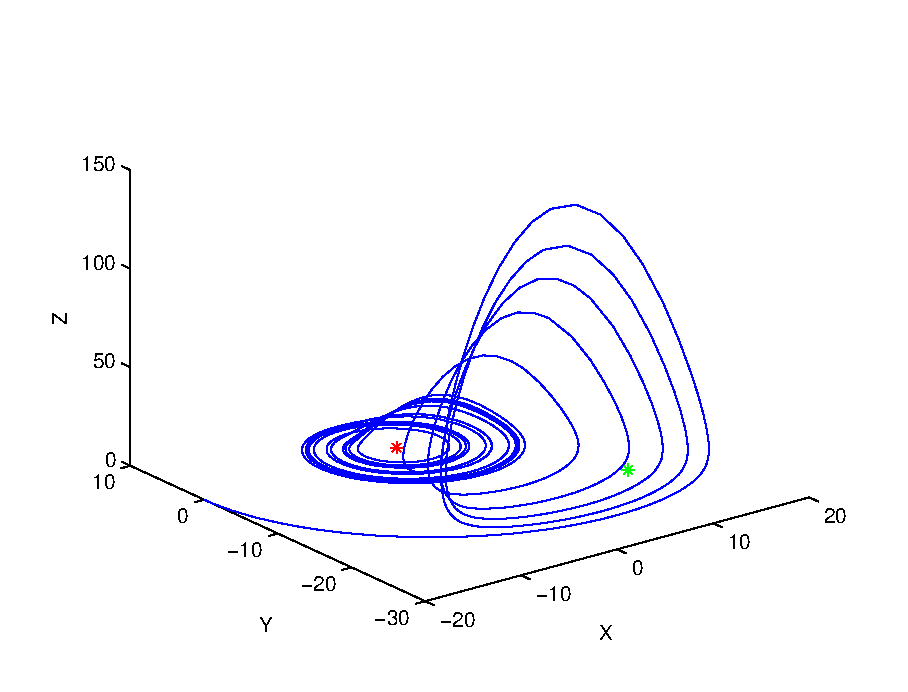
\includegraphics[width=0.7\columnwidth]{chapter3Fig/3d.eps}\\
	% 
	\caption{罗塞尔吸引子的变化情况}\label{Fig: rossler三维}	
	
\end{figure}

罗塞尔吸引子的各项参数设定为:$  a_1=0.2 $, $ a_2=0.2 $,$ a_3=5 $。
则稳定点为:$ \overline{\textbf{x}}=(0.008, -0.040, 0.040)^T $。
本实验中,节点间的耦合强度耦合强度$ c=0.3 $,节点间的耦合方式设定为$ H = [1,0,0;0,0,0;0,0,0] $,可以计算出$ \alpha_1 $与$ \alpha_2 $的值。如图 \ref{Fig: rossler} , $ (\alpha_2,\alpha_1)=(-4.991, -0.192) $。
此外,控制节点的反馈强度$ d $为网络节点的最大度减$ 1 $,即$ d = k_{max}-1 $。


\begin{figure}[ht]%{.5\linewidth}
	\centering
	% Requires \usepackage{graphicx}
	\includegraphics[width=0.5\columnwidth]{chapter3Fig/rossler.eps}\\
	% 
	\caption{最大特征值$ \Lambda_{max}$ 关于$\alpha$的函数曲线 }
	\label{Fig: rossler}	
	
\end{figure}

\subsubsection{实验结果}
图 \ref{Fig: opt_r} 描述了$ 4 $个真实网络中,传统判据$ R $、耦合强度范围$ \omega $和收敛速度$ v $最优的情况下,传统判据$ R $随控制节点比例$ \theta $的变化情况。
首先,可以明显看到,不存在两条趋势线是完全重叠的;也就是说,传统判据,耦合强度范围和收敛速度这三个指标确实是三个不同的指标,他们从不同角度去刻画了网络的牵制控制。
传统判据$ R $越大代表网络更容易受控,到达稳定状态。
在图中,随着牵制控制节点的增加,不同控制节点集合对应的传统判据也在不断地增加,节点对网络的控制能力也越强。
最后,可以看到随着控制节点比例的增加,红色线$ R_{opt} $和黑色线$ \omega_{opt} $这两个集合相差不大,但都优于蓝色线$ v_{opt} $。
尤其是在\ref{Fig: opt_r} (a) PDZBase 网络中,$ v_{opt} $和$ \omega_{opt} $差别很大。

\begin{figure}[htbp]%{.5\linewidth}
	\centering
	% Requires \usepackage{graphicx}
	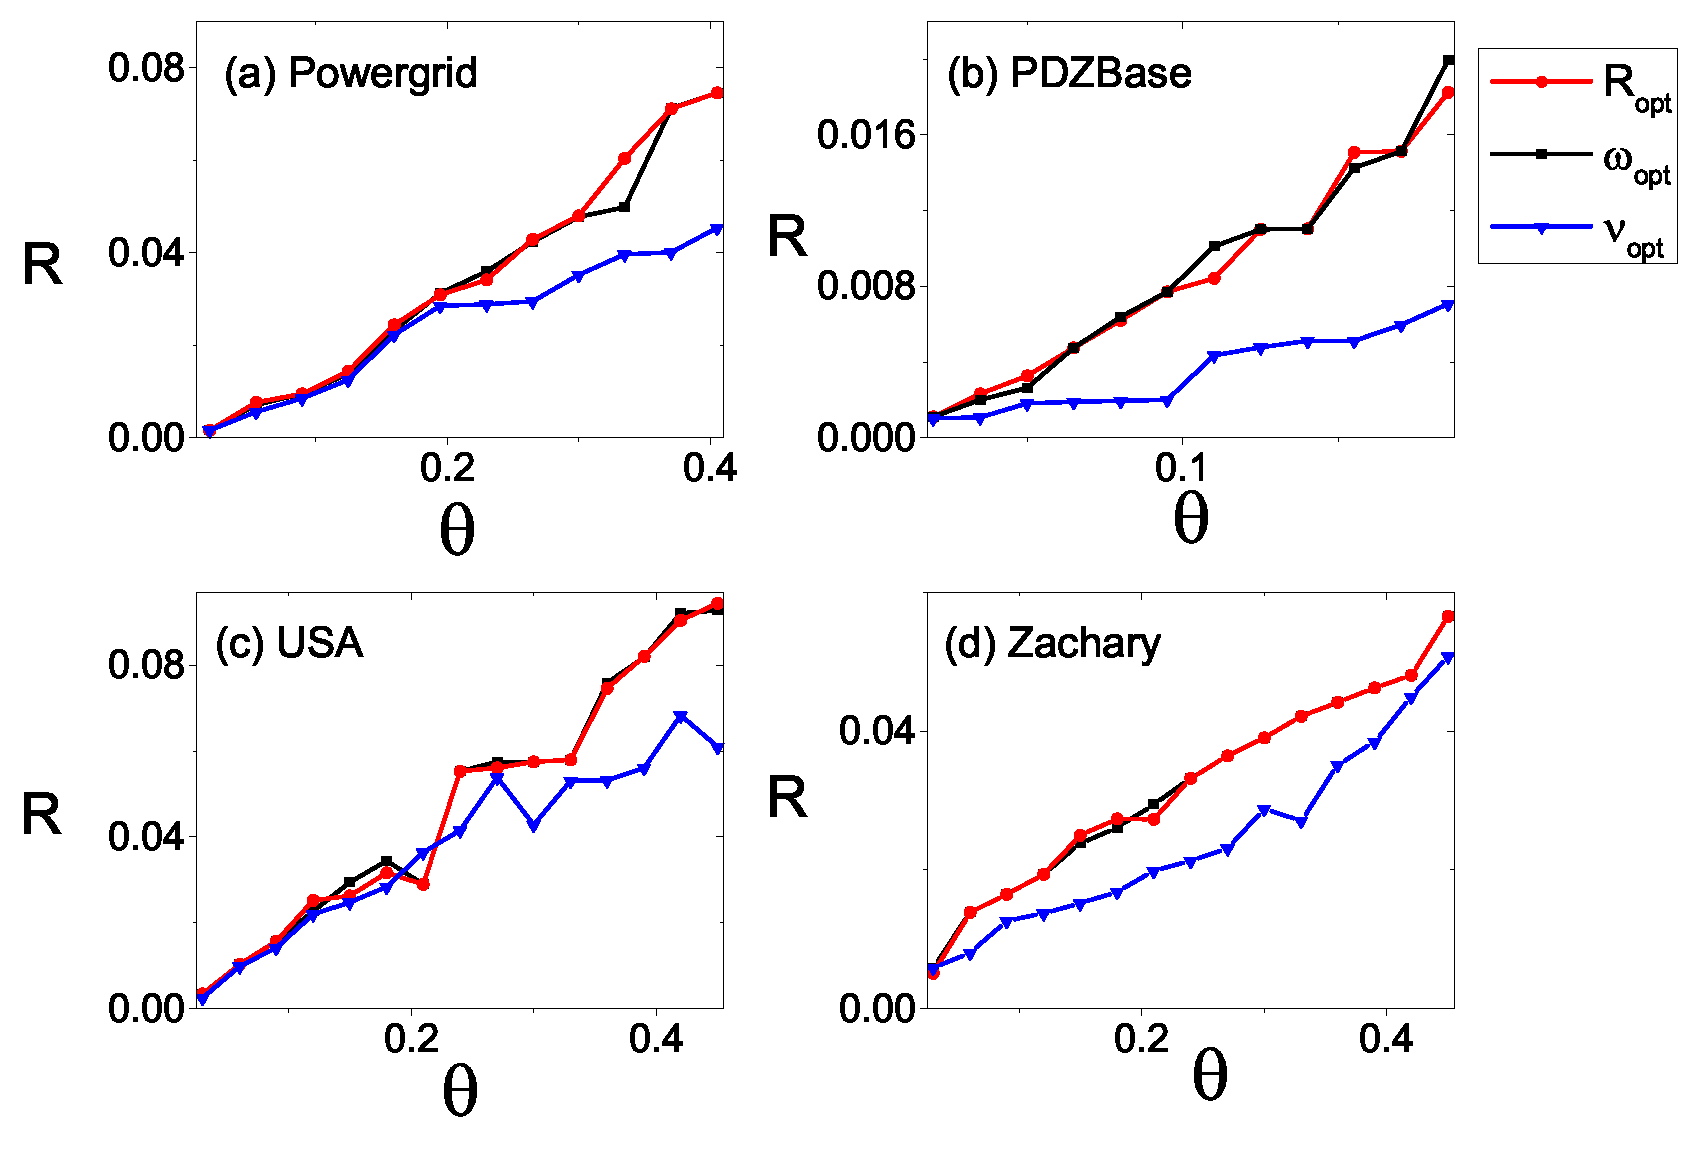
\includegraphics[width=0.9\columnwidth]{chapter3Fig/R.eps}\\
	% 
	\caption{不同网络中传统判据随控制节点比例的变化情况}
	\label{Fig: opt_r}	
	
\end{figure}

\begin{figure}[hp]%{.5\linewidth}
	\centering
	% Requires \usepackage{graphicx}
	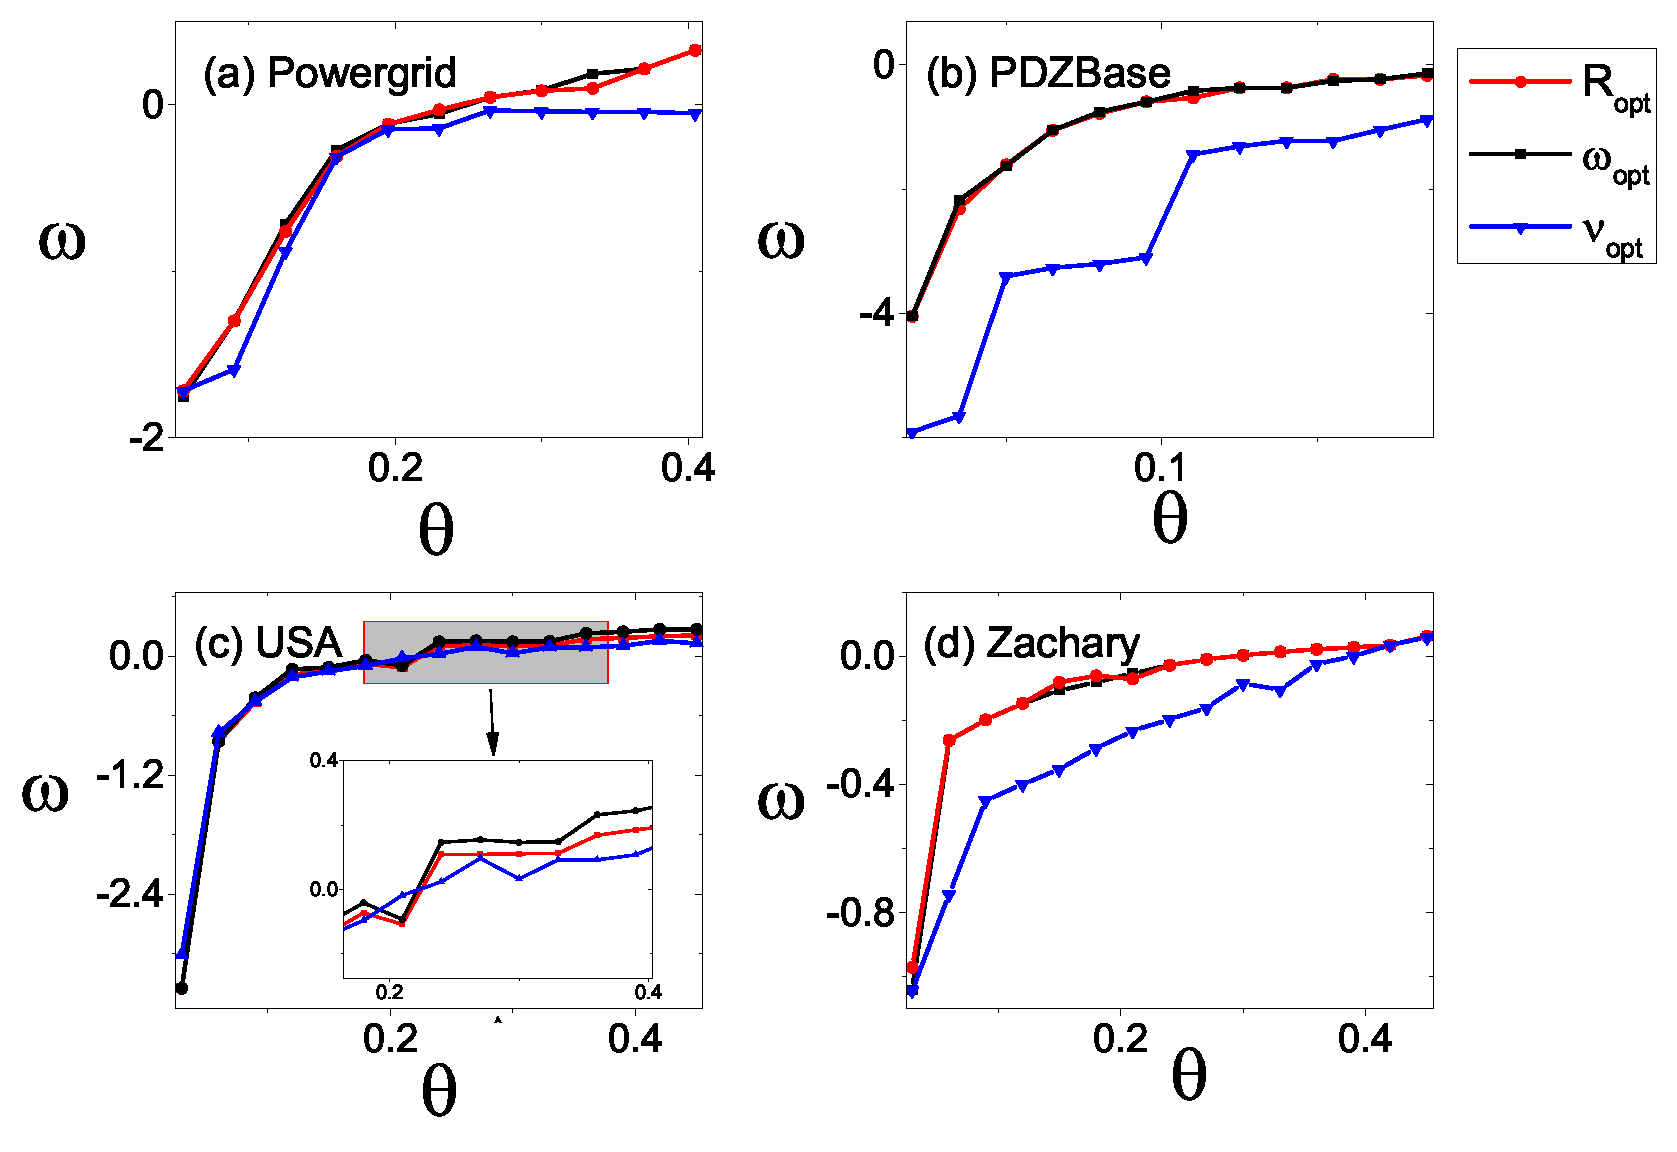
\includegraphics[width=0.9\columnwidth]{chapter3Fig/W.eps}\\
	% 
	\caption{不同网络中耦合强度范围随控制节点比例的变化情况}
	\label{Fig: opt_W}	
	
\end{figure}

\begin{figure}[hp]%{.5\linewidth}
	\centering
	% Requires \usepackage{graphicx}
	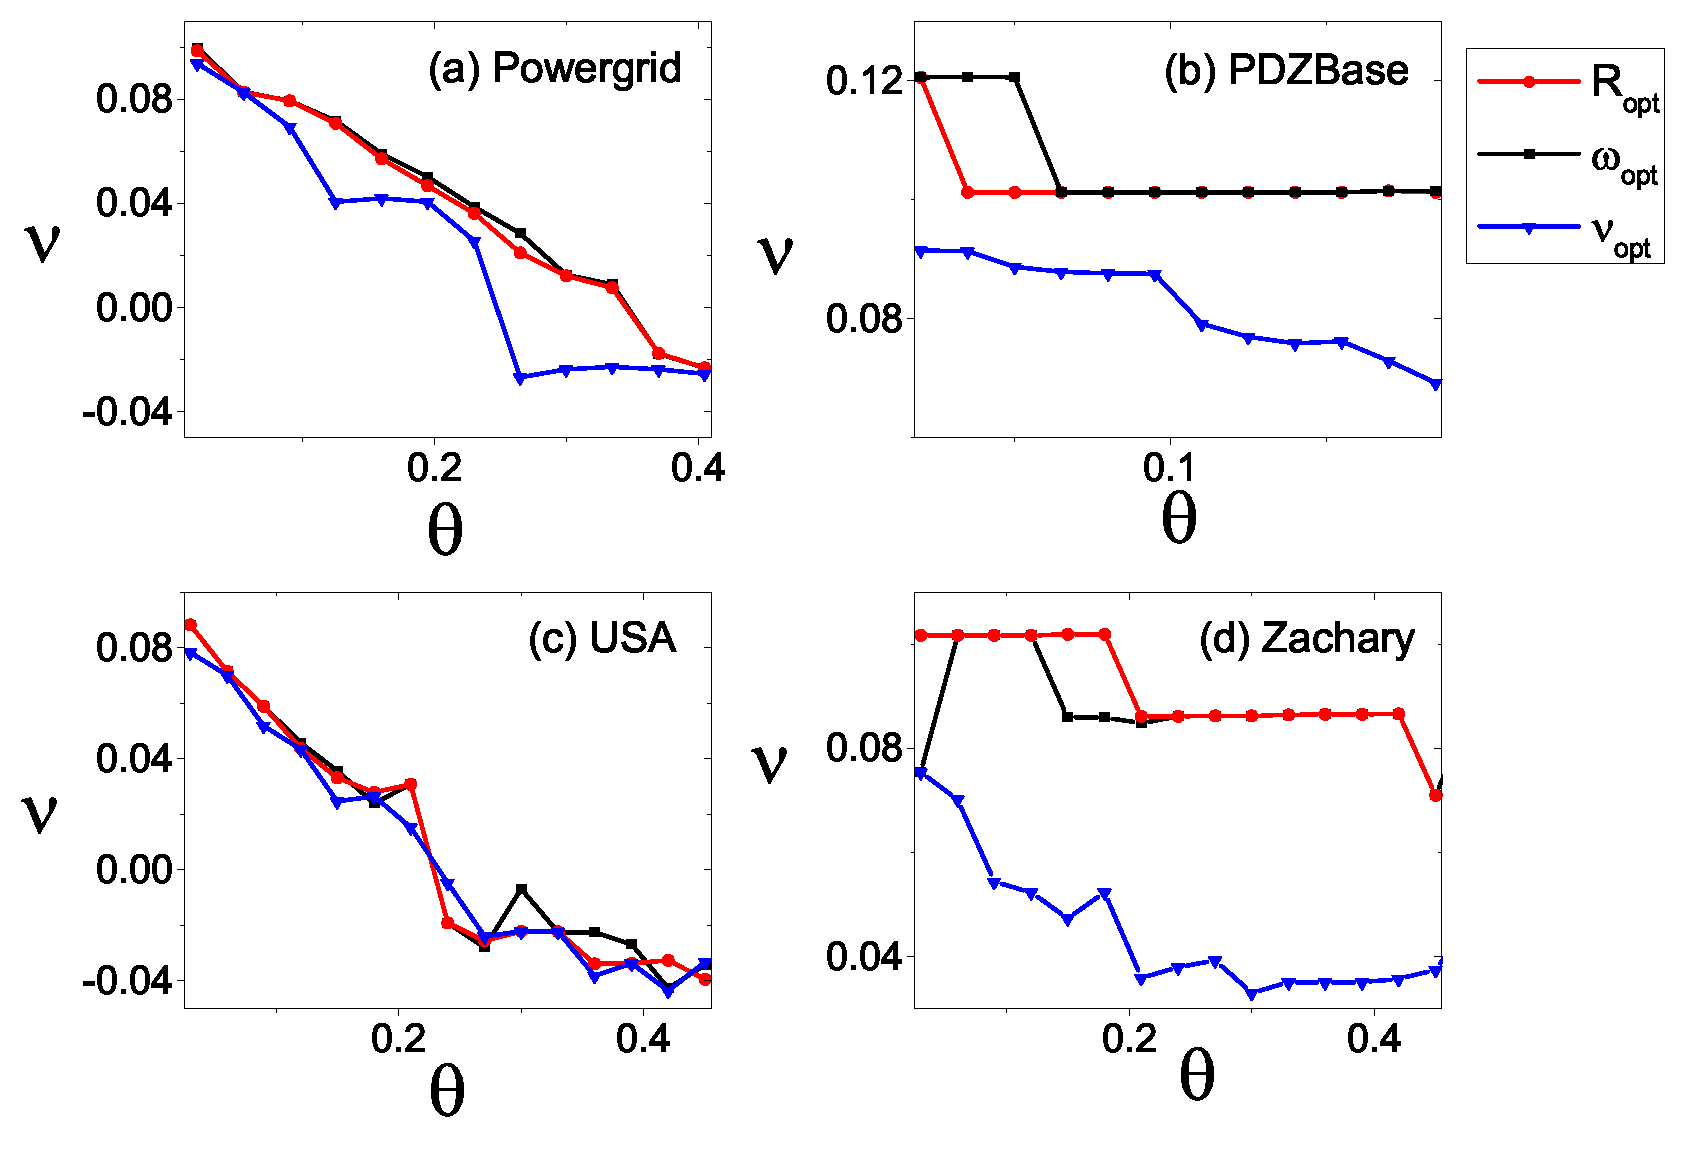
\includegraphics[width=0.9\columnwidth]{chapter3Fig/V.eps}\\
	% 
	\caption{不同网络中收敛速度随控制节点比例的变化情况}
	\label{Fig: opt_V}	
	
\end{figure}

\begin{figure}[hp]%{.5\linewidth}
	\centering
	% Requires \usepackage{graphicx}
	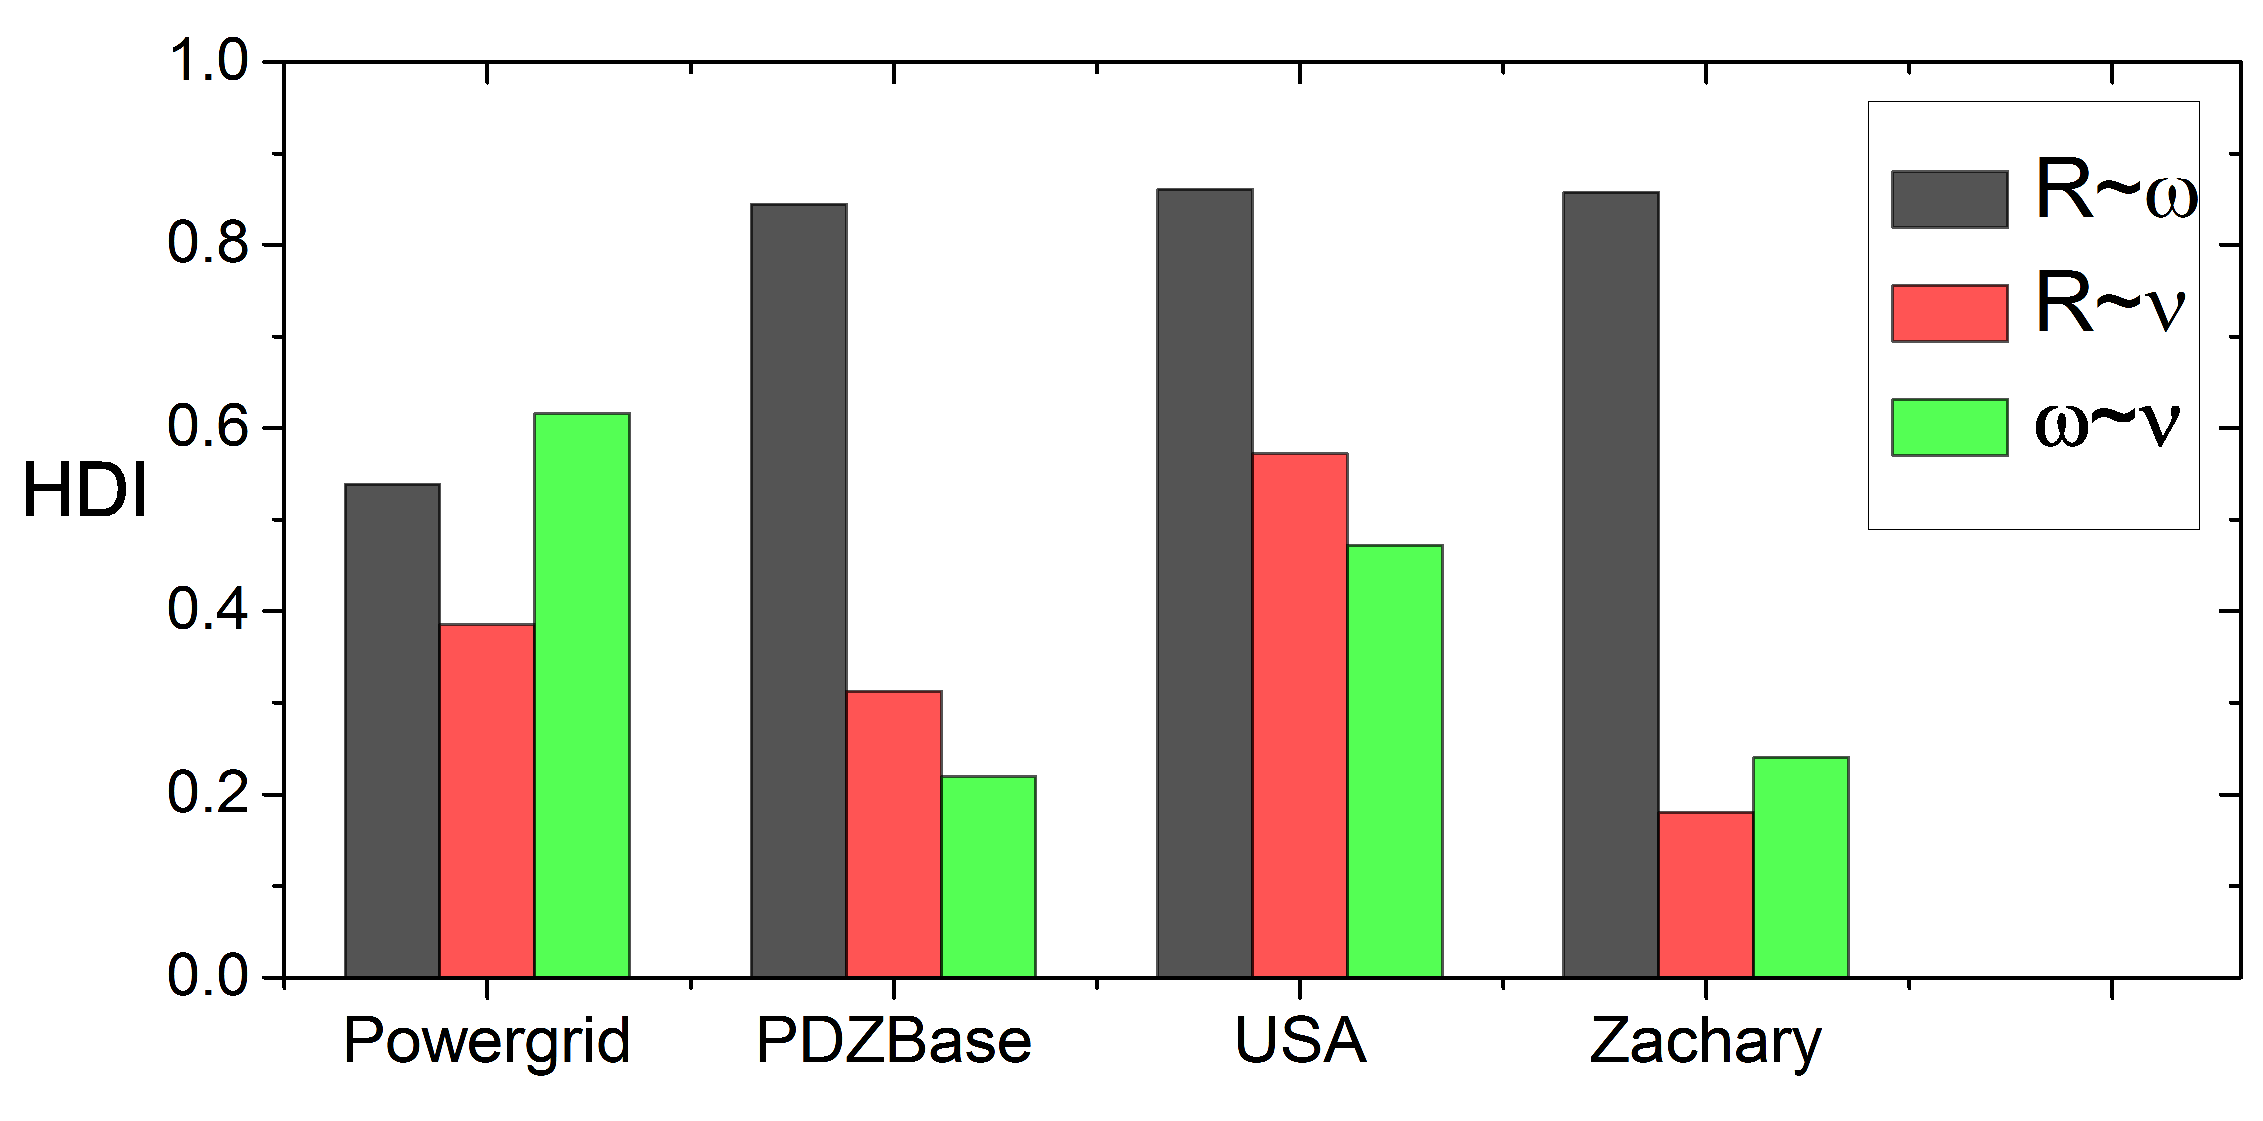
\includegraphics[width=0.8\columnwidth]{chapter3Fig/overlap.eps}\\
	% 
	\caption{不同网络中三个指标的重叠情况}
	\label{Fig: chap2overlap}		
\end{figure}

图 \ref{Fig: opt_W} 和图 \ref{Fig: opt_V} 分别描述了耦合强度范围和收敛速度随控制节点比例的变化情况。
在图 \ref{Fig: opt_W}中,耦合强度范围越大,网络更容易受控到达稳定状态。与图\ref{Fig: R}类似,红色线$ R_{opt} $和黑色线$ \omega_{opt} $相差不大,并且优于蓝色线$ v_{opt} $。
在图 \ref{Fig: opt_V}中,收敛速度$ v<0 $,且越小越好。图中可以明显看出蓝色线$ v_{opt} $优于红色线$ R_{opt} $和黑色线$ \omega_{opt} $。
可以从图 \ref{Fig: opt_r}、图 \ref{Fig: opt_W} 和图 \ref{Fig: opt_V}中归纳出,不存在一个控制节点集合(一条颜色线),同时在经典判据$ R $、耦合强度范围$ \omega $和收敛速度$ v $中达到最优。
另外需要注意的是,在图 \ref{Fig: opt_V} (a) Powergrid 网络 中,当控制节点比例$ \theta<0.2 $时,该网络的收敛速度$ v>0 $,这意味着系统中有一个正的李雅普诺夫指数,即该系统无法到达稳定状态。


总体而言,传统判据、耦合强度范围和收敛速度三个评价指标是无法同时达到最优。但是,红色线$ R_{opt} $和黑色线$ \omega_{opt} $在图 \ref{Fig: opt_r}和图 \ref{Fig: opt_W}中相差不大。这是否意味着经典判据和耦合强度范围存在比较强的相关性呢?

接下来,实验取20\%的结点作为牵制控制节点,观察不同网络中,这三个指标选择控制节点的重叠情况。如图\ref{Fig: chap2overlap},在PDZBase、USA、Zachary网络中,$ {\rm HDI}_{R~\omega}>0.8 $,这说明耦合强度范围和传统判据这两个指标在这几个网络中,相似性非常高;相比较而言,$ {\rm HDI}_{R~v} $与$ {\rm HDI}_{\omega~v} $较低一些。
需要注意的是,$ R $、$ \omega $和$ v $是三个不同的衡量指标,他们分别从不同角度去说明了网络的牵制控制问题。



\subsection{本章小结}
本章从经典网络控制问题出发,提出了衡量节点对网络牵制控制的传统比率判据。但实验发现,传统判据无法精确描述牵制控制,因此提出了耦合强度范围和收敛速度两个指标。前者决定了网络受控稳定时耦合强度的大小,后者则从网络的拓扑结构方面,给出了系统受控稳定时的收敛速度。同时,本章在理论上分析了传统判据、耦合强度范围和收敛速度无法同时到达最优,并在实验中给出了验证。


\clearpage
